\chapter{Methodology}
\label{ch:methodology}

\section{Overview}
\label{sec:method-overview}

This thesis develops and evaluates diffusion-based neural solvers for routing problems. The proposed methodology follows a two-stage training pipeline. First, a DIFUSCO-style graph diffusion model is trained with supervised denoising using solver-generated reference solutions \citep{sun2023difusco}. Second, the supervised checkpoint can be further adapted using a CADO-style reinforcement learning objective that directly rewards the quality of the decoded solution \citep{yoon2024cado}.

The motivation for this design is that supervised denoising provides stable training for high-dimensional binary solution structures, while reinforcement learning fine-tuning reduces the mismatch between the training objective and the final evaluation objective. In supervised learning, the model is trained to imitate reference binary labels. However, routing performance is ultimately determined only after the predicted heatmap is passed through a non-differentiable decoder. Therefore, the second stage explicitly incorporates the decoder and the decoded solution cost into the training signal.

\begin{figure}[htbp]
    \centering
    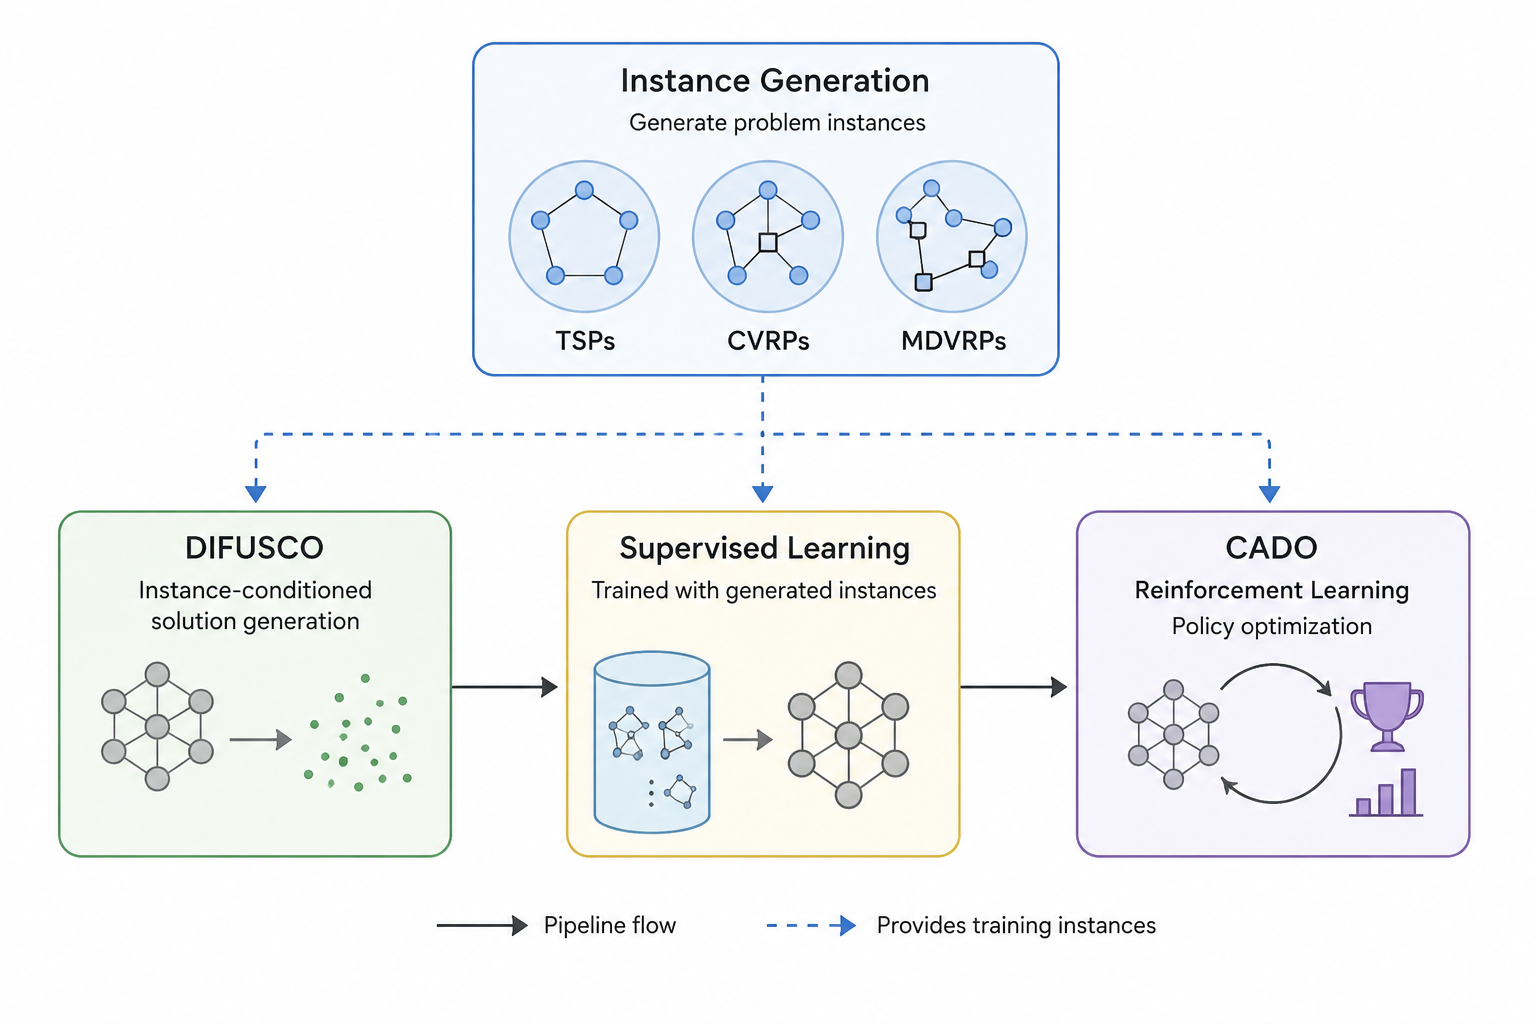
\includegraphics[width=0.85\textwidth]{./figures/pipeline.png}
    \caption{
        Overview of the proposed training and evaluation pipeline. A DIFUSCO-style diffusion model is first trained by supervised denoising on solver-generated binary labels \citep{sun2023difusco}. The trained checkpoint can then be fine-tuned with a CADO-style reinforcement learning objective based on decoded solution quality \citep{yoon2024cado}.
    }
    \label{fig:pipeline}
\end{figure}

The implementation covers three routing settings: the Traveling Salesman Problem (TSP), the Capacitated Vehicle Routing Problem (CVRP), and the Multi-Depot Vehicle Routing Problem (MDVRP). For TSP, the model predicts a heatmap over candidate tour edges. For CVRP, the same edge-heatmap formulation is extended to multi-route vehicle routing by adding depot and demand information to the node representation and by enforcing capacity during decoding. For MDVRP, this thesis considers an assignment-level formulation in which the model predicts customer--depot assignment scores. Therefore, TSP and CVRP are evaluated using decoded route cost and relative gap to a reference solution, whereas MDVRP is evaluated using assignment-level metrics such as depot-assignment accuracy and capacity-violation rate.

\section{Binary Solution Representation}
\label{sec:binary-solution-representation}

Following the graph-based diffusion formulation of DIFUSCO \citep{sun2023difusco}, each optimization instance is represented by a binary solution vector. Let \(s\) denote a problem instance and let
\[
    x_0 \in \{0,1\}^{|\mathcal{B}_s|}
\]
denote the clean binary solution label, where \(\mathcal{B}_s\) is the set of candidate binary decisions for instance \(s\). The meaning of each binary variable depends on the problem setting.

For TSP, \(\mathcal{B}_s\) consists of candidate edges between cities. A variable \(x_{ij}=1\) indicates that edge \((i,j)\) is included in the tour. A feasible decoded solution must form a Hamiltonian cycle in which every city has degree two and all cities belong to a single connected tour.

For CVRP, \(\mathcal{B}_s\) consists of candidate arcs between the depot and customers. A variable \(x_{ij}=1\) indicates that a vehicle travels directly from node \(i\) to node \(j\). A feasible decoded solution must visit every customer exactly once, start and end each route at the depot, and ensure that the total demand assigned to each vehicle route does not exceed the vehicle capacity \(Q\).

For MDVRP, this thesis uses an assignment-level binary representation. Let \(D\) be the set of depots and \(C\) be the set of customers. The binary variable
\[
    x_{di} =
    \begin{cases}
    1, & \text{if customer } i \text{ is assigned to depot } d,\\
    0, & \text{otherwise}
    \end{cases}
\]
represents a customer--depot assignment decision. A feasible assignment should assign every customer to exactly one depot and should not exceed the available aggregate capacity of each depot. This representation captures the higher-level decision in MDVRP, but it does not directly construct the vehicle routes within each depot. After assignment, a full MDVRP solution would still require solving one CVRP subproblem for each depot.

\section{Discrete Diffusion Training}
\label{sec:discrete-diffusion-training}

The supervised training stage follows the discrete diffusion process used for graph-based combinatorial optimization in DIFUSCO \citep{sun2023difusco}. Starting from a clean reference solution \(x_0\), the forward process gradually corrupts the binary variables into noisy states \(x_t\) for timesteps \(t=1,\ldots,T\). In the discrete Bernoulli diffusion setting, each binary variable is represented as a two-class categorical variable. The transition matrix at timestep \(t\) is
\[
    Q_t =
    \begin{pmatrix}
    1-\beta_t & \beta_t \\
    \beta_t & 1-\beta_t
    \end{pmatrix},
\]
where \(\beta_t\) is the corruption probability. Thus, the forward transition is defined as
\[
    q(x_t \mid x_{t-1})
    =
    \mathrm{Cat}
    \left(
        x_t;
        p=\tilde{x}_{t-1}Q_t
    \right),
\]
where \(\tilde{x}_{t-1}\) denotes the one-hot representation of \(x_{t-1}\).

During training, a timestep \(t\) is sampled, the corresponding noisy solution \(x_t\) is generated, and the denoising network predicts the clean binary label \(x_0\). The network receives the problem instance \(s\), the noisy binary state \(x_t\), and the timestep \(t\), and returns two-class logits for each candidate decision:
\[
    z_\theta = f_\theta(s,x_t,t).
\]
The supervised denoising objective is the cross-entropy loss between the predicted logits and the clean reference solution:
\[
    \mathcal{L}_{\mathrm{SL}}(\theta)
    =
    \mathbb{E}_{s,x_0,t,x_t}
    \left[
        \frac{1}{|\mathcal{B}_s|}
        \sum_{b \in \mathcal{B}_s}
        \mathrm{CE}
        \left(
            z_{\theta,b}, x_{0,b}
        \right)
    \right].
\]
The probability assigned to class 1 is interpreted as the heatmap value:
\[
    A_b
    =
    P_\theta(x_{0,b}=1 \mid s,x_t,t)
    =
    \mathrm{softmax}(z_{\theta,b})_1.
\]
This heatmap is later decoded into a feasible or repaired discrete solution.

\section{Graph Denoising Architecture}
\label{sec:graph-denoising-architecture}

The denoising model is implemented as an edge-aware graph neural network following the AGNN-style backbone used in DIFUSCO \citep{sun2023difusco}. The backbone maintains both node embeddings and edge embeddings, which is important because the main prediction target in routing problems is edge-based or assignment-edge-based.

The TSP model receives node coordinates, edge indices, edge distances, the noisy edge state \(x_t\), and the diffusion timestep \(t\). The initial node representation is obtained from a sinusoidal positional embedding of the two-dimensional coordinates:
\[
    h_i^{(0)} = \phi_{\mathrm{pos}}(p_i),
\]
where \(p_i=(x_i,y_i)\) is the coordinate of city \(i\). The initial edge representation is the concatenation of a distance embedding and a noisy-state embedding:
\[
    e_{ij}^{(0)}
    =
    \left[
        \phi_{\mathrm{dist}}(d_{ij});
        \phi_{\mathrm{noise}}(x_{t,ij})
    \right],
\]
where \(d_{ij}\) is the Euclidean distance between nodes \(i\) and \(j\).

For CVRP, the node representation is extended to include demand and depot information. Each node feature is defined as
\[
    u_i =
    [x_i, y_i, q_i/Q, \mathbb{I}(i=\mathrm{depot})],
\]
where \(q_i\) is the demand of node \(i\), \(Q\) is the vehicle capacity, and \(\mathbb{I}(i=\mathrm{depot})\) indicates whether the node is the depot. This means that capacity information is available to the neural network through the normalized demand feature \(q_i/Q\). However, the supervised objective remains an edge-wise denoising loss and does not explicitly penalize capacity violations. Capacity feasibility is handled by the decoder and evaluation procedure.

For MDVRP, the node representation is
\[
    u_i =
    [x_i, y_i, q_i/Q, r_i],
\]
where \(r_i\) is a role indicator distinguishing depot nodes from customer nodes. The same edge-denoising backbone is used, but the candidate edge set is restricted to customer--depot assignment edges in the MDVRP experiment. Thus, the MDVRP model predicts assignment heatmaps rather than complete route structures.

The timestep \(t\) is embedded using a sinusoidal timestep embedding and projected through a small multilayer perceptron:
\[
    \tau_t = \mathrm{MLP}_{t}(\mathrm{Embed}(t)).
\]
At each AGNN layer, node and edge embeddings are updated jointly:
\[
    (H^{(\ell+1)}, E^{(\ell+1)})
    =
    \mathrm{AGNNLayer}
    \left(
        H^{(\ell)}, E^{(\ell)}, \mathcal{E}, \tau_t
    \right),
\]
where \(\mathcal{E}\) is the candidate edge or assignment-edge set. After the final layer, an edge-level classification head maps each final edge embedding to two logits:
\[
    z_{ij}
    =
    \mathrm{MLP}_{\mathrm{edge}}
    \left(
        e_{ij}^{(L)}
    \right).
\]
The resulting class-1 probabilities form the heatmap used for decoding.

\section{Problem-Specific Decoding}
\label{sec:problem-specific-decoding}

The diffusion model produces heatmap scores, but heatmaps do not automatically satisfy the hard constraints of routing problems. Therefore, each problem requires a problem-specific decoder that maps the predicted scores into a feasible or repaired solution.

For TSP, the decoder ranks undirected candidate edges using the sum of the two directed heatmap scores normalized by Euclidean distance, as in heatmap decoding for DIFUSCO \citep{sun2023difusco}. Edges are inserted into the partial solution only if they do not violate degree constraints and do not create a premature subtour. The process continues until a complete Hamiltonian cycle is formed. A local search heuristic such as 2-opt \citep{croes1958method} can optionally be applied to improve the decoded tour; in the evaluation code, 2-opt is applied to the decoded TSP tour.

For CVRP, the decoder uses a similar score-ranked edge insertion procedure. Customer nodes are constrained to degree two, customer-only subtours are forbidden, and capacity feasibility is enforced by tracking the demand of each partial customer chain before it is connected to the depot. If some customers remain open after the greedy pass, they are attached to the depot as a repair step. The decoded CVRP cost is the sum of Euclidean distances over all recovered vehicle routes.

For MDVRP, the decoder operates on the customer--depot assignment heatmap. The directed scores for each customer--depot pair are averaged into an assignment score matrix. Customers are then processed in descending order of confidence, measured by the margin between the best depot score and the median depot score. Each customer is assigned to the highest-scoring depot with enough remaining aggregate capacity. If no depot has enough remaining capacity, the customer is assigned to the depot with the largest remaining capacity and this forced assignment is counted as an over-capacity event. Since this experiment stops at the assignment stage, it does not construct depot-specific vehicle routes. Consequently, MDVRP is evaluated using assignment-level metrics rather than full MDVRP routing cost.

\section{CADO-Style Reinforcement Learning Fine-Tuning}
\label{sec:cado-style-finetuning}

The supervised denoising objective trains the model to imitate solver-generated reference solutions. However, minimizing cross-entropy against reference labels does not necessarily minimize the cost of the final decoded solution. This mismatch occurs because the supervised loss is not aware of the non-differentiable decoder and does not directly optimize the routing objective. To reduce this mismatch, this thesis applies CADO-style reinforcement learning fine-tuning after supervised pretraining \citep{yoon2024cado}.

Let \(g_s(\cdot)\) denote the problem-specific decoder and let \(C_s(\cdot)\) denote the decoded solution cost. The reverse diffusion process is treated as a Markov decision process. At denoising timestep \(t\), the state contains the instance, the timestep, and the current noisy solution:
\[
    \sigma_t = (s,t,x_t).
\]
The action is the next denoised sample:
\[
    a_t = x_{t-1}.
\]
The policy is the learned reverse transition:
\[
    \pi_\theta(a_t \mid \sigma_t)
    =
    p_\theta(x_{t-1} \mid x_t,s).
\]

In implementation, fine-tuning does not roll out all \(T\) diffusion steps. Instead, a shorter inference schedule of \(M_{\mathrm{train}}\) steps is sampled, starting from Bernoulli noise \(x_T \sim \mathrm{Bernoulli}(0.5)\). The stochastic posterior transitions before the last scheduled step produce the actions and log probabilities used for policy-gradient training. At the final scheduled step, the predicted class-1 probabilities are thresholded to obtain the binary heatmap. The heatmap is then decoded into a solution:
\[
    \hat{x}
    =
    g_s(A_\theta).
\]
For TSP and CVRP, the reward is defined as the negative decoded route cost:
\[
    R_{\mathrm{SR}}
    =
    -C_s(\hat{x}).
\]
This is the standard reward formulation. Lower-cost decoded solutions receive higher rewards. The implemented rewards do not add an explicit violation penalty. Instead, feasibility is mainly handled by the decoders, and remaining violations are reported as evaluation metrics.

When a reference solution cost is available, this thesis also considers a label-centered reward:
\[
    R_{\mathrm{LCR}}
    =
    -
    \left(
        C_s(\hat{x}) - C_s(x^{\mathrm{ref}})
    \right).
\]
Here, \(C_s(x^{\mathrm{ref}})\) serves as an instance-dependent baseline. Since this baseline depends only on the problem instance and not on the sampled denoising trajectory, it reduces variance without changing the expected policy-gradient direction.

For MDVRP, the current implementation does not use a route-cost reward because the model predicts only customer--depot assignments. The reward is instead the negative assignment miss rate,
\[
    R_{\mathrm{MDVRP}}
    =
    -
    \left(
        1
        -
        \mathrm{Acc}_{\mathrm{assign}}
    \right).
\]
In this assignment-level setting, the SR and LCR modes both use the same negative miss-rate reward.

The REINFORCE gradient estimator \citep{williams1992simple} is estimated as
\[
    \nabla_\theta J(\theta)
    =
    \mathbb{E}
    \left[
        A
        \sum_{m=1}^{M_{\mathrm{train}}-1}
        \nabla_\theta
        \bar{\ell}_{m}
    \right],
\]
where \(A\) is the scalar advantage and \(\bar{\ell}_{m}\) is the mean Bernoulli log probability of the sampled transition at scheduled step \(m\). For TSP and CVRP, this mean is taken over all candidate edges. For MDVRP, it is taken only over customer--depot bipartite edges, so that customer--customer context edges do not dilute the assignment-learning signal. In SR mode, the advantage is the batch-standardized reward. In LCR mode for TSP and CVRP, the centered reward \(R_{\mathrm{LCR}}\) is used directly as the advantage.

The implemented REINFORCE loss is
\[
    \mathcal{L}_{\mathrm{RL}}
    =
    -
    A
    \sum_{m=1}^{M_{\mathrm{train}}-1}
    \bar{\ell}_{m}
    -
    0.01
    \left(
        -
        \frac{1}{B}
        \sum_{i=1}^{B}
        \sum_{m=1}^{M_{\mathrm{train}}-1}
        \bar{\ell}_{i,m}
    \right),
\]
where \(B\) is the accumulated batch size. The second term is a sampled negative-log-probability bonus used as a practical exploration proxy; it is not a separately computed Shannon entropy of the full reverse-transition distribution.

\section{Hybrid Fine-Tuning Strategy}
\label{sec:hybrid-finetuning-strategy}

Fine-tuning the entire diffusion backbone with reinforcement learning can be unstable and memory-intensive. To improve stability, this thesis uses the supervised checkpoint as the initialization for RL fine-tuning. The fine-tuning stage updates only the parameters selected for adaptation while preserving most of the representation learned during supervised denoising.

In the hybrid fine-tuning setting, all parameters are frozen first. The final AGNN layers selected for adaptation and the edge-classification head are then fully unfrozen. In the earlier AGNN layers, low-rank adapters \citep{hu2022lora} are inserted into the linear maps \(P\), \(Q\), \(R\), \(U\), and \(V\), while the original base weights remain frozen. For a base linear map \(W\), the adapted computation has the form
\[
    Wx
    +
    \frac{1}{r}
    W_{\mathrm{up}}
    W_{\mathrm{down}}
    x,
\]
where \(r\) is the LoRA rank. In the experiments, the default configuration uses rank \(r=2\) and fully updates the last graph layer together with the output head. This design reflects the intuition that early graph layers capture reusable geometric and relational features, whereas the final layers are more responsible for producing the heatmap that interacts with the decoder. The same fine-tuning interface supports ablations over reward type, algorithm choice, and the number of denoising steps.

\section{Evaluation Metrics}
\label{sec:evaluation-metrics}

The evaluation protocol depends on the output space of each problem. During evaluation, the model uses deterministic generation with \(M_{\mathrm{eval}}\) scheduled denoising steps, rather than the stochastic rollout used to collect RL trajectories.

For TSP, the primary metric is the decoded tour length. When a reference solution is available, the relative gap is computed as
\[
    \mathrm{Gap}(\%)
    =
    \frac{
        C_{\mathrm{model}} - C_{\mathrm{ref}}
    }{
        C_{\mathrm{ref}}
    }
    \times 100.
\]
Here, \(C_{\mathrm{model}}\) is the cost of the decoded model solution and \(C_{\mathrm{ref}}\) is the cost of the reference solution. If the reference solution is solver-generated but not proven optimal, this metric is interpreted as a relative gap to the reference solution rather than a true optimality gap.

For CVRP, the decoded cost is the total length of all vehicle routes. The same relative gap formula is used. In addition, feasibility is checked by counting decoded routes whose load exceeds the vehicle capacity \(Q\). The reported over-capacity rate is the average number of over-capacity routes per evaluated instance.

For MDVRP, the model output is a depot-assignment heatmap. Therefore, the evaluation uses assignment-level metrics. Depot-assignment accuracy is defined as
\[
    \mathrm{Acc}_{\mathrm{assign}}
    =
    \frac{1}{|C|}
    \sum_{i \in C}
    \mathbb{I}
    \left(
        \hat{d}(i) = d^{\mathrm{ref}}(i)
    \right),
\]
where \(\hat{d}(i)\) is the predicted depot for customer \(i\), and \(d^{\mathrm{ref}}(i)\) is the reference depot assignment. The MDVRP decoder attempts to avoid aggregate depot-capacity violations during assignment. If a customer must be assigned when no depot has enough remaining capacity, the decoder records a forced over-capacity assignment. The reported capacity-violation rate is
\[
    \mathrm{ViolRate}
    =
    \frac{
        N_{\mathrm{overcap}}
    }{
        |C|
    },
\]
where \(N_{\mathrm{overcap}}\) is the number of customers that were forced into an over-capacity depot during decoding. For diagnostic analysis, one can also compute depot-level excess demand,
\[
    \mathrm{Excess}
    =
    \frac{1}{|D|}
    \sum_{d \in D}
    \frac{
        \max
        \left(
            0,
            \sum_{i \in C:\hat{d}(i)=d} q_i - m_d Q
        \right)
    }{
        m_d Q
    }.
\]
These metrics reflect the intended scope of the MDVRP experiment: evaluating whether the diffusion model can learn meaningful customer--depot assignments under capacity constraints.